\documentclass[a4paper]{article}
\usepackage[english]{babel}
\usepackage[utf8x]{inputenc}
\usepackage[T1]{fontenc}
\usepackage[a4paper,top=3cm,bottom=2cm,left=3cm,right=3cm,marginparwidth=1.75cm]{geometry}
\usepackage{amsmath}
\usepackage[colorinlistoftodos]{todonotes}
\usepackage[utf8]{inputenc}
\usepackage[vietnam,english,french]{babel}
\usepackage{natbib}
\usepackage{graphicx}
\usepackage{amsmath}
\usepackage{amsfonts}
\usepackage{amssymb}
\usepackage[T1,T5]{fontenc} 
\usepackage[utf8]{inputenc}
\usepackage[vietnam,english,french]{babel}
\usepackage[a4paper,top=3cm,bottom=2cm,left=3cm,right=3cm,marginparwidth=1.75cm]{geometry}
\usepackage{amsmath}
\usepackage[colorinlistoftodos]{todonotes}
\input{pd1supp.def}
\usepackage{amsmath,amsxtra,amssymb,amsthm,latexsy m,amscd,amsfonts}
\usepackage[tcvn]{inputenc}
\usepackage[T1,T5]{fontenc}
\usepackage[utf8]{inputenc}
\usepackage[vietnam,english,french]{babel}
\usepackage[dvips]{color}
\usepackage{graphicx}
\usepackage{color}
\usepackage{colortbl}
\usepackage{amsfonts}
\usepackage{amssymb}
\usepackage{tabularx}
\usepackage{makecell}

\documentclass[a4paper]{article}
\usepackage{vntex}
%\usepackage[english,vietnam]{babel}
\usepackage[utf8]{vietnam}

%\usepackage[utf8]{inputenc}
%\usepackage[francais]{babel}
\usepackage{a4wide,amssymb,epsfig,latexsym,multicol,array,hhline,fancyhdr}

\usepackage{amsmath}
\usepackage{lastpage}
\usepackage[lined,boxed,commentsnumbered]{algorithm2e}
\usepackage{enumerate}
\usepackage{color}
\usepackage{graphicx}							% Standard graphics package
\usepackage{array}
\usepackage{tabularx, caption}
\usepackage{multirow}
\usepackage{multicol}
\usepackage{rotating}
\usepackage{graphics}
\usepackage{geometry}
\usepackage{setspace}
\usepackage{epsfig}
\usepackage{tikz}
\usetikzlibrary{arrows,snakes,backgrounds}
\usepackage{hyperref}
\hypersetup{urlcolor=blue,linkcolor=black,citecolor=black,colorlinks=true} 
%\usepackage{pstcol} 								% PSTricks with the standard color package
\graphicspath{ {./images/} }


%\usepackage{fancyhdr}
\setlength{\headheight}{40pt}
\pagestyle{fancy}
\fancyhead{} % clear all header fields
\fancyhead[L]{
 \begin{tabular}{rl}
    \begin{picture}(25,15)(0,0)
    \put(0,-8){
\includegraphics[width=8mm, height=8mm]{hcmut.png}}
    %\put(0,-8){\epsfig{width=10mm,figure=hcmut.eps}}
   \end{picture}&
	%
\includegraphics[width=8mm, height=8mm]{hcmut.png} & %
	\begin{tabular}{l}
		\textbf{\bf \ttfamily Trường Đại Học Bách Khoa Tp.Hồ Chí Minh}\\
		\textbf{\bf \ttfamily Khoa Khoa Học và Kỹ Thuật Máy Tính}
	\end{tabular} 	
 \end{tabular}
}
\fancyhead[R]{
	\begin{tabular}{l}
		\tiny \bf \\
		\tiny \bf 
	\end{tabular}  }
\fancyfoot{} % clear all footer fields
\fancyfoot[L]{\scriptsize \ttfamily BÁO CÁO BÀI TẬP LỚN}
\fancyfoot[R]{\scriptsize \ttfamily Trang {\thepage}/\pageref{LastPage}}
\renewcommand{\headrulewidth}{0.3pt}
\renewcommand{\footrulewidth}{0.3pt}


%%%
\setcounter{secnumdepth}{4}
\setcounter{tocdepth}{3}
\makeatletter
\newcounter {subsubsubsection}[subsubsection]
\renewcommand\thesubsubsubsection{\thesubsubsection .\@alph\c@subsubsubsection}
\newcommand\subsubsubsection{\@startsection{subsubsubsection}{4}{\z@}%
                                     {-3.25ex\@plus -1ex \@minus -.2ex}%
                                     {1.5ex \@plus .2ex}%
                                     {\normalfont\normalsize\bfseries}}
\newcommand*\l@subsubsubsection{\@dottedtocline{3}{10.0em}{4.1em}}
\newcommand*{\subsubsubsectionmark}[1]{}
\makeatother


\begin{document}

\begin{titlepage}
\begin{center}
ĐẠI HỌC QUỐC GIA THÀNH PHỐ HỒ CHÍ MINH \\
TRƯỜNG ĐẠI HỌC BÁCH KHOA \\
KHOA KHOA HỌC - KỸ THUẬT MÁY TÍNH 
\end{center}

\vspace{1cm}

\begin{figure}[h!]
\begin{center}

\includegraphics[width=3cm]{hcmut.png}
\end{center}
\end{figure}

\vspace{1cm}


\begin{center}
\begin{tabular}{c}
\multicolumn{1}{c}{\textbf{{\Large KIỂM TRA PHẦN MỀM}}}\\
\hline
\\
\multicolumn{1}{c}{\textbf{{ BÁO CÁO BÀI TẬP LỚN}}}\\
\multicolumn{1}{c}{\textbf{{\Large World Cup}}}\\
~~\\
\hline
\end{tabular}
\end{center}

\vspace{2cm}

\begin{table}[h]
\begin{tabular}{rrl}
\hspace{5 cm} 
& GVHD: & Băng Ngọc Bảo Tâm \\
& Nhóm: & 1\\
& SV: & Huỳnh Quốc Phú  - 1712638 \\
& & Hy Phạm Ngọc Linh - 1711947\\
& & Trương Gia Bảo  - 1710019\\
& & Trần Minh Tú  -1713850\\
\end{tabular}
\end{table}
\begin{center}
{\footnotesize TP. HỒ CHÍ MINH, THÁNG 11/2019}
\end{center}
\end{titlepage}
\newpage

\tableofcontents
% \newpage \listoffigures
% \newpage \listoftables
\newpage
\section{Giới thiệu:}\\
\hspace{0.5cm}Tài liệu này trình bày quá trình xây dựng, cách thức hoạt động của chương trình mô phỏng bài toán World Cup cùng với các kiểm thử của nó theo mô hình Test - Driven Development (TDD).
\section{Tìm hiểu về mô hình TTD:}\\
\hspace{0.5cm}Test-driven development (TDD) là một cách tiếp cận để phát triển kết hợp test đầu tiên. Bạn sẽ viết test trước khi bạn viết đầy đủ code để hoàn thành việc test và refactoring. Mục tiêu của TDD là một cách suy nghĩ để thông qua các yêu cầu hoặc thiết kế trước khi viết code các chức năng của hệ hống (TDD là một kĩ thuật quan trọng cả yêu cầu agile và thiết kế agile). Quan điểm khác, TDD là một kỹ thuật lập trình giúp viết code hoạt động sạch sẽ.\\\\
\textbf{ TDD là gì?}\\
\hspace{0.5cm}Các bước đầu tiên của phát triển test-first (TFD) được mô tả trong diagram hoạt động UML ở hình dưới đây. Đầu tiên, nhanh chóng add một test , đủ đơn giản để code fail. Bước tiếp theo là chạy các test, thường xuyên hoàn thành test mặc dù chỉ chạy các subset sẽ đem lại tốc độ cao hơn, để chắc chắn rằng new test trên thực tế là fail. Sau đó, bạn cần update functional code để làm nó pass qua các test mới. Bước thứ tư là chạy lại test một lần nữa. Nếu chúng fail, bạn lại tiếp tục update functional code và retest. Mỗi lần test pass bước tiếp theo là bắt đầu lại (đầu tiên bạn có thể cần refector bất kì sao chép nào trong design của bạn, chuyển từ TFD sang TDD).\\\\
\textbf{ Các bước trong Test-First Development (TFD)}\\
\begin{center}
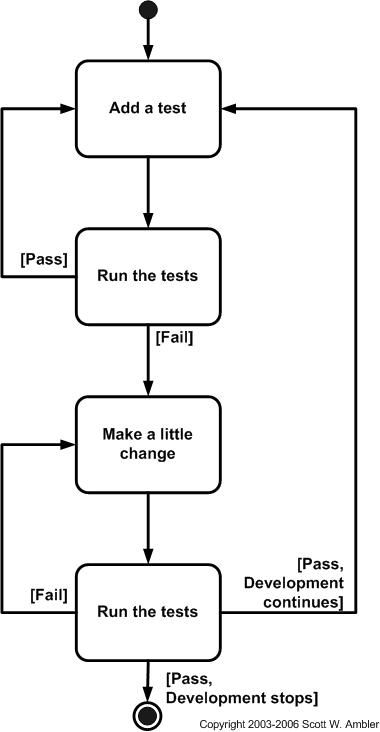
\includegraphics[scale=0.5]{hinh1.jpg}    
\end{center}
Ta có thể hiểu TDD với công thức đơn giản sau:\textbf{ TDD = refectoring + TFD}

TDD hoàn toàn xoay quanh development truyền thống. Đầu tiên khi bạn thực thi chức năng mới, câu hỏi đầu tiên mà bạn đề cập về design phải là một bản design tốt nhất có thể cho phép bạn triển khai được không. Nếu có bạn tiến hành thông qua cách tiếp cận TFD. Nếu không, bạn refactor cục bộ để thay đổi phần design bị ảnh hưởng bở chức năng mới, cho phép bạn thêm chức năng mới một cách dễ dàng. Kết quả là bạn sẽ luôn luôn cải thiện được chức năng của design, do đó ta sẽ dễ dàng làm việc hơn trong tương lai.

Thay vì viết code chức năng đầu tiên và sau đó mới thực thi testing code sau, nếu bạn viết lại tất cả, thay vào đó bạn biết test code trước khi viết functional code. Hơn nữa, bạn làm như vậy trong các bước rất nhỏ – một test và một ít functional code tương ứng tại một thời điểm. Một programmer thực hiện một phương pháp tiếp cận TDD từ chối viết một hàm mới cho đến khi có first test fails vì không có chức năng đó. Trong thực tế, họ từ chối thêm ngay cả một dòng code duy nhất cho đến khi một test tồn tại. Khi test đã được thực hiện, họ sẽ thực hiện yêu cầu công việc để đảm bảo pass các test. Điều này nghe đơn giản về nguyên tắc, nhưng khi bạn lần đầu tiên học tập để có một cách tiếp cận TDD , nó yêu cầu một kỉ luật tuyệt vời bời vì rất dễ bỏ qua và viết mã code mà không cần viết một test mới. Một trong những lợi thế của lập trình pair là pair của bạn sẽ giúp bạn theo dõi điều đó.

Có hai level của TDD:
\begin{itemize}
    \item \textbf{Acceptance TDD (ATDD):} Với ATDD bạn viết một single acceptance test duy nhất, hoặc behavioral specification tùy thuộc vào thuật ngữ ưa thích của bạn, và sau đó chỉ đủ hiệu suất để thực thi code để hoàn thành test đó. Mục tiêu của ATDD là xác định các yêu cầu chi tiết, thực thi cho giải pháp của bạn trên cơ sở thời gian (JIT). ATDD còn được gọi là Behavior Driven Development (BDD).
    \item \textbf{Developer TDD:} Với developer TDD, bạn viết một single developer test, đôi khi được gọi không chính xác là một unit test, và sau đó chỉ cần đủ production code để hoàn thành test đó. Mục tiêu của developer TDD là chỉ định thiết kế chi tiết, thực thi cho giải pháp của bạn dựa trên cơ sở JIT. Developer TDD thường được gọi là TDD. Hình sau đây mô tả diagram hoạt động của UML cho thấy ATDD and developer TDD kết hợp với nhau như thế nào. Một cách lý tưởng, bạn sẽ viết một single acceptance test, sau đó thực hiện production code được yêu cầu để hoàn thành test đó, bạn sẽ thực hiện phương pháp TDD của developer. Điều này lần lượt yêu cầu bạn phải lặp lại nhiều lần việc viết test, viết production code, làm nó theo một chu kì làm việc theo developer TDD level.
\end{itemize}
\textbf{Cách acceptance TDD and developer TDD làm việc với nhau.}
\begin{center}
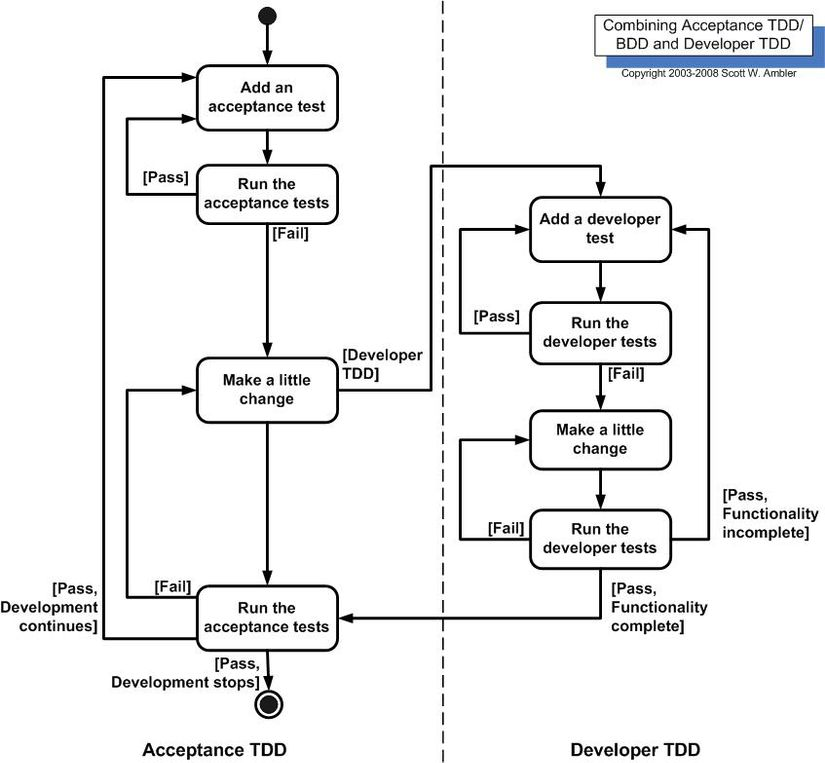
\includegraphics[scale=0.5]{hinh2.jpg}    
\end{center}
Lưu ý rằng Hình trên đây giả định rằng bạn đang làm cả hai, mặc dù có thể làm một trong hai mà không có sự khác biệt. Trên thực tế, một số đội sẽ làm developer TDD mà không thực hiện ATDD, mặc dù nếu bạn đang thực hiện ATDD thì chắc chắn bạn đang làm developer TDD. Thách thức ở đây là cả hai dạng của TDD đều yêu cầu các học viên phải có kỹ năng kỹ năng testing kỹ thuật, các kỹ năng mà nhiều chuyên gia yêu cầu thường không có.

\textbf{Testing thông qua xUnit Framework.}
\begin{center}
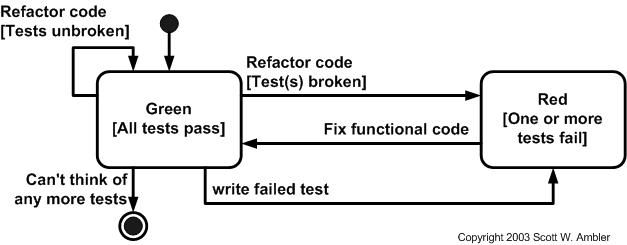
\includegraphics[scale=0.5]{hinh3.jpg}    
\end{center}
Kent Beck, người đã phổ biến TDD trong chương trình eXtreme (XP) (Beck 2000), định nghĩa hai quy tắc đơn giản cho TDD (Beck 2003). Trước tiên, ạn chỉ nên viết business code mới khi một automated test tự động fail. hứ hai, bạn nên loại bỏ bất kỳ trùng lặp mà bạn tìm thấy. Beck giải thích hai nguyên tắc đơn giản này tạo ra hành vi cá nhân và nhóm phức tạp như thế nào:
\begin{itemize}
\item Bạn phát triển cơ bản, với running code cung cấp phản hồi giữa các quyết định.
\item Bạn viết tests bởi vì bạn không thể đợi 20 lần mỗi ngày để người khác viết chúng cho bạn.
\item Môi trường phát triển của bạn phải đáp ứng nhanh những thay đổi nhỏ
\item Thiết kế của bạn phải bao gồm các thành phần liên kết chặt chẽ và lỏng lẻo để làm cho việc testing dễ dàng hơn Đối với các developer, họ cần phải học cách viết unit test có hiệu quả. Kinh nghiệm của Beck’s experience dể có unit test tốt:
\item Chạy nhanh (chúng có thiết lập ngắn, run times, và break downs).
\item Chạy trong sự cô lập (bạn sẽ có thể sắp xếp lại chúng).
\item Sử dụng dữ liệu giúp chúng dễ đọc và dễ hiểu.
\item Sử dụng dữ liệu thực khi cần
\item Đạt được một bước về mục tiêu chung của bạn.
\end{itemize}
\section{Mô tả project của nhóm:}\\
\subsection{Database:}\\

\hspace{0.5cm}Tổ chức lưu trứ thông tin trong cơ sở dữ liệu SQL đi kèm chương trình
\begin{center}
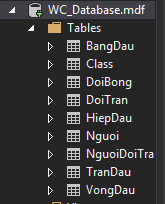
\includegraphics[scale=1.3]{hinh4.png}    
\end{center}
\subsection{Mô tả hoạt động xử lí giải World Cup:}\\

\hspace{0.5cm}Số lượng các đội bóng của mỗi khu vực được đưa vào database ban đầu như sau:
\begin{itemize}
\item Khu vực châu Á: 6 đội
\item Khu vực châu Phi: 5 đội
\item Khu vực châu Bắc, Trung Mỹ và Caribe: 4 đội
\item Khu vực Nam Mỹ: 4 đội
\item Khu vực Châu Đại dương: 1 đội
\item Khu vực Châu Âu: 13 đội
\item Đội chủ nhà
\end{itemize}

Đội bóng đứng thứ 6 khu vực châu Á sẽ đá 2 trận play-off với đội bóng đứng thứ 4 khu vực châu Bắc, Trung Mỹ và Caribe để giành suất sự vòng chung kết. Đội bóng đứng thứ 4 khu vực Nam Mỹ sẽ đá 2 trận play-off với đội bóng đứng thứ 1 khu vực châu Đại Dương để giành suất sự vòng chung kết. Sau vòng này số lượng đội bóng mỗi khu vực như sau:
\begin{itemize}
\item Khu vực châu Á: 5.5 đội
\item Khu vực châu Phi: 5 đội
\item Khu vực châu Bắc, Trung Mỹ và Caribe: 3.5 đội
\item Khu vực Nam Mỹ: 3.5 đội
\item Khu vực Châu Đại dương: 0.5 đội
\item Khu vực Châu Âu: 13 đội
\item Đội chủ nhà
\end{itemize}

32 đội bóng vào vòng chung kết được chia làm 8 bảng đấu theo thứ tự từ A-H, mỗi bảng có 4 đội bóng được đánh số thứ tự 1-4.

Ở vòng bảng, các đội trong cùng bảng đấu sẽ thi đấu vòng tròn một lượt tính điểm. Tỉ số mỗi trận sẽ được random và lưu lại vào database. Kết quả sẽ được tính dựa trên hiệu số bàn thắng - thua mỗi trận.

2 đội cao điểm nhất mỗi bảng sẽ được đưa vào vòng trong.

Ở vòng tiếp theo 1/16, các đội được sắp xếp thi đấu như sau:
\begin{itemize}
\item Trận 1: Nhất bảng A – Nhì bảng B
\item Trận 2: Nhất bảng B – Nhì bảng A
\item Trận 3: Nhất bảng C – Nhì bảng D
\item Trận 4: Nhất bảng D – Nhì bảng C
\item Trận 5: Nhất bảng E – Nhì bảng F
\item Trận 6: Nhất bảng F – Nhì bảng E
\item Trận 7: Nhất bảng G – Nhì bảng H
\item Trận 8: Nhất bảng H – Nhì bảng G
\end{itemize}

Các trận đấu được random kết quả tỉ số và được tính toán thắng thua chỉ dựa vào kết quả tỉ số, không tính hiệp phụ, luân lưu, không kiểm tra số lượng cầu thủ trên sân,… và được lưu vào database.

8 đội thắng ở vòng 1/16 sẽ được tiếp tục xử lí đấu vòng tứ kết như sau:
\begin{itemize}
\item Trận Q1: Thắng trận 1 – Thắng trận 2
\item Trận Q2: Thắng trận 3 – Thắng trận 4
\item Trận Q3: Thắng trận 5 – Thắng trận 2
\item Trận Q4: Thắng trận 7 – Thắng trận 8
\end{itemize}

Các trận đấu được random kết quả tỉ số và được tính toán thắng thua chỉ dựa vào kết quả tỉ số, không tính hiệp phụ, luân lưu, không kiểm tra số lượng cầu thủ trên sân,… và được lưu vào database

4 đội thắng ở vòng tứ kết sẽ được tiếp tục xử lí đấu vòng bán kết như sau:
\begin{itemize}
\item Trận S1: Thắng trận Q1 – Thắng trận Q2
\item Trận S2: Thắng trận Q3 – Thắng trận Q4
\end{itemize}

Các trận đấu được random kết quả tỉ số và được tính toán thắng thua chỉ dựa vào kết quả tỉ số, không tính hiệp phụ, luân lưu, không kiểm tra số lượng cầu thủ trên sân,… và được lưu vào database.

Hai đội giành chiến thắng ở vòng bán kết sẽ gặp nhau ở trận chung kết để tranh cúp vô địch. Trận đấu được random kết quả tỉ số và được tính toán thắng thua chỉ dựa vào kết quả tỉ số, không tính hiệp phụ, luân lưu, không kiểm tra số lượng cầu thủ trên sân,… và được lưu vào database.
\subsection{Mô tả các class hiện thực}
\begin{itemize}
\item \textbf{BangDau.cs:} \\
Lưu thông tin ID bảng đấu đánh số từ 1 đến 8 tương ứng với “A”-“H”, danh sách các đội bóng và danh sách các trận đấu trong khuôn khổ vòng bảng.\\
Cho phép khởi tạo với đội bóng truyền vào và kiểm tra số đội bóng hợp lệ mỗi bảng(4 đội).
\item \textbf{Vong16.cs:}\\
Lưu thông tin các đội bóng được vào vòng 1 - 16, danh sách các trận đấu và lưu các đội được đi tiếp đến vòng tứ kết.\\
\item \textbf{VongTuKet.cs:}\\
Lưu thông tin 8 đội bóng lọt vào vòng tứ kết, đồng thời là bốn trận đấu của vòng tứ kết và kết quả các đội được đi tiếp.\\
\item \textbf{VongBanKet.cs:}\\
Lưu thông tin các đội bóng được vào vòng bán kết, danh sách các trận đấu và lưu các đội được đi tiếp đến vòng cuối cùng là chung kết.\\
\item \textbf{VongChungKet.cs:}\\
Lưu hai đội bóng duy nhất lọt vào chung kết, trận đấu chung kết, và đội lên ngôi vô địch kì World Cup này.\\
\item \textbf{Database.cs:}\\
Xử lý dữ liệu database cho toàn bộ project.
\item \textbf{DoiBong.cs:}\\
Lưu 1 số thông tin cần thiết của đội bóng như ID, khu vực, danh sách thành viên, danh sách cầu thủ,…
\item \textbf{DoiTran.cs:}\\
Lưu và xử lí 1 đội trong 1 trận duy nhất, cập nhật dữ liệu database và kiểm tra 1 số ràng buộc về số cầu thủ mỗi đội.
\item \textbf{TranDau.cs:}\\
Lưu các thông tin như 2 đội trong 1 trận, tỉ số,… \\
Xử lý kết quả trận đấu, cập nhật dữ liệu cho database
\item \textbf{Nguoi.cs:}\\
Lưu các thông tin như ID, tên, vai trò(HLV, cầu thủ), số bàn thắng, điểm(nếu là cầu thủ)…\\
Cập nhật database
\end{itemize}
Chi tiết các class được thể hiện trong Class - Diagram sau : 
\begin{center}
    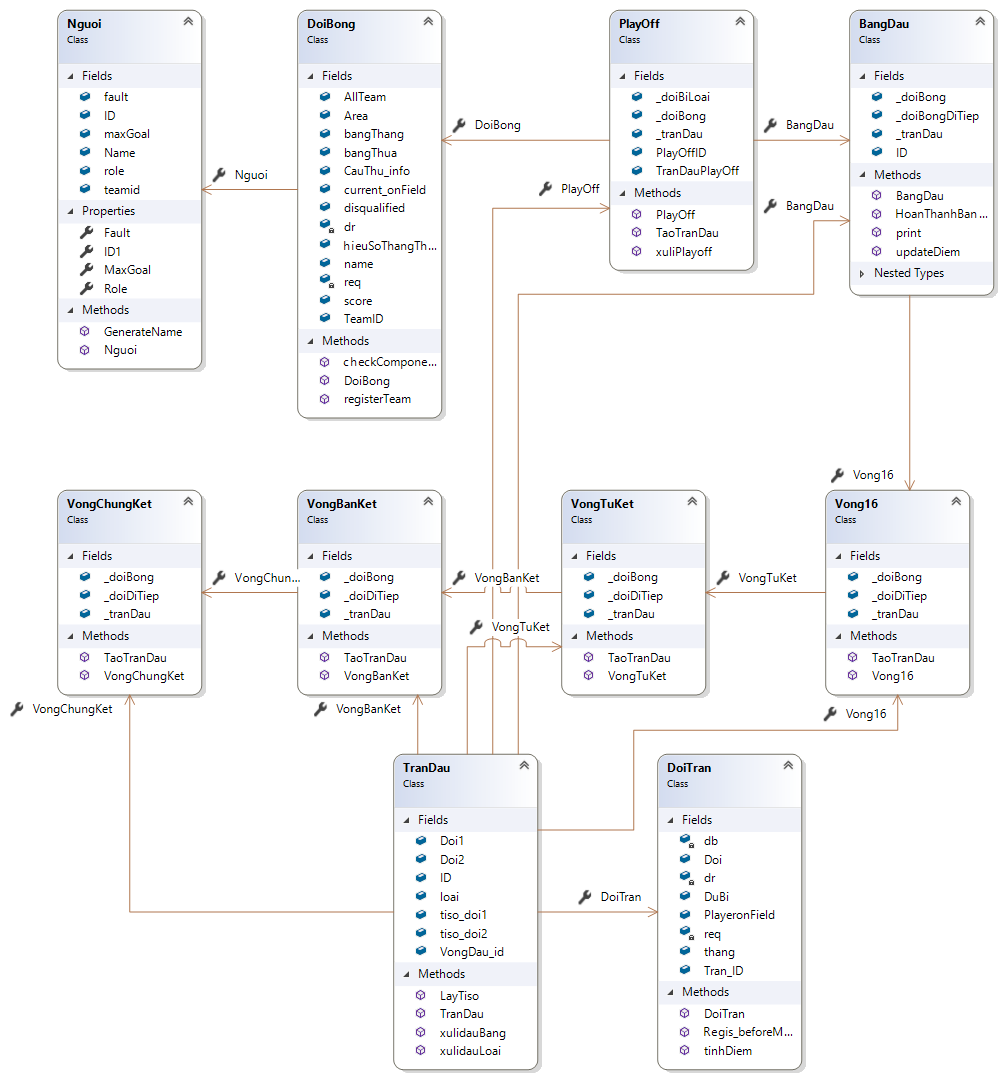
\includegraphics[scale=0.6]{WorldCup_ClassDiagram.png}  \\ 
\end{center}
\subsection{Môi trường kiểm tra:}\\
\hspace{0.5cm}Hiện thực trên C\#

Dùng tiện ích Nunit 2.6.4 để hiện thực unit-test theo các testcase được định nghĩa.

Ứng dụng chạy tốt trên các phiên bản windows xp, windows 7, windows 8,  windows 10.
\section{Mẫu 1 số testcase để kiểm thử:}\\
\subsection{TestBangDau.cs:}
Dùng để test class BangDau.cs\\

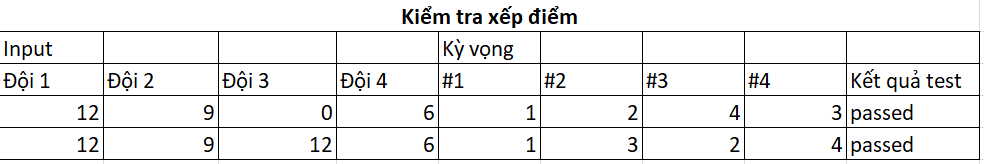
\includegraphics[scale=0.45]{hinh6.png}  \\ 

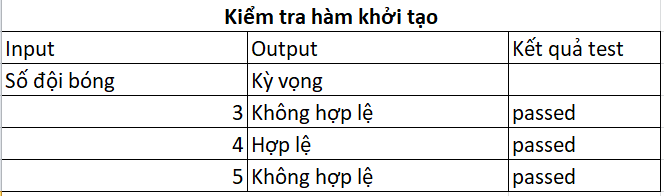
\includegraphics[scale=0.5]{hinh5.png}\\

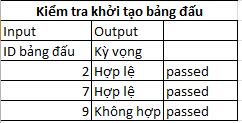
\includegraphics[scale=0.8]{hinh7.png}\\


\subsection{TestDoiBong.cs}
Dùng để test class DoiBong.cs\\

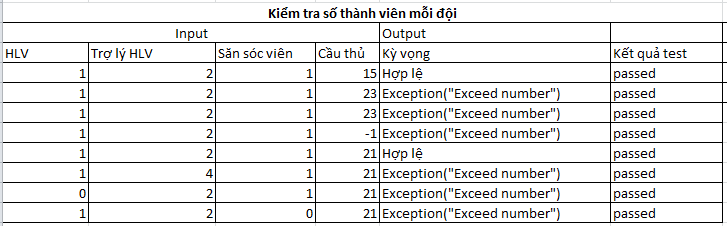
\includegraphics[scale=0.6]{hinh9.png}  \\ 

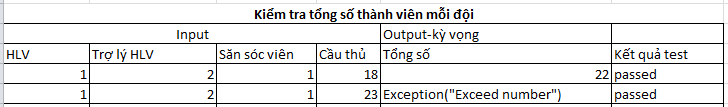
\includegraphics[scale=0.5]{hinh10.png}\\

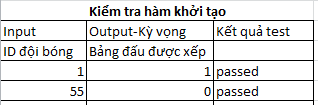
\includegraphics[scale=0.8]{hinh8.png}\\

\subsection{TestDoiTran.cs}
Dùng để test class DoiTran.cs\\

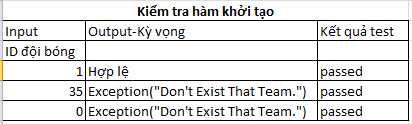
\includegraphics[scale=0.8]{hinh11.png}  \\ 

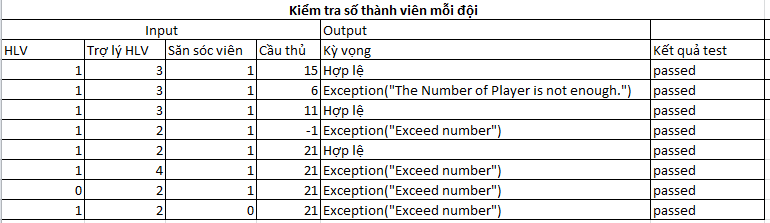
\includegraphics[scale=0.5]{hinh13.png}\\

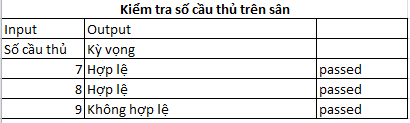
\includegraphics[scale=0.8]{hinh12.png}\\

\subsection{TestTranDau.cs}
Dùng để test class TranDau.cs\\

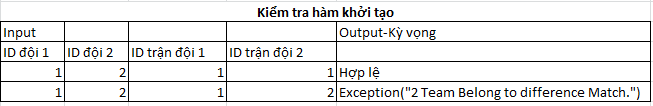
\includegraphics[scale=0.7]{hinh14.png}  \\ 

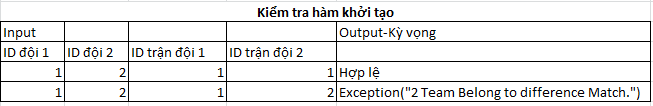
\includegraphics[scale=0.7]{hinh14.png}\\


\section{Những testcase chưa kiểm tra:}\\
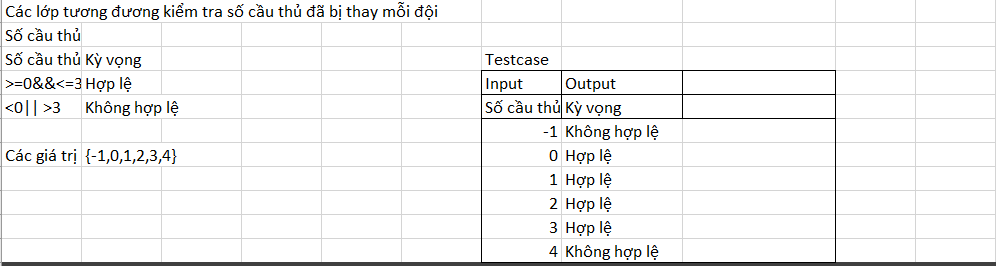
\includegraphics[scale=0.75]{hinh16.png}\\
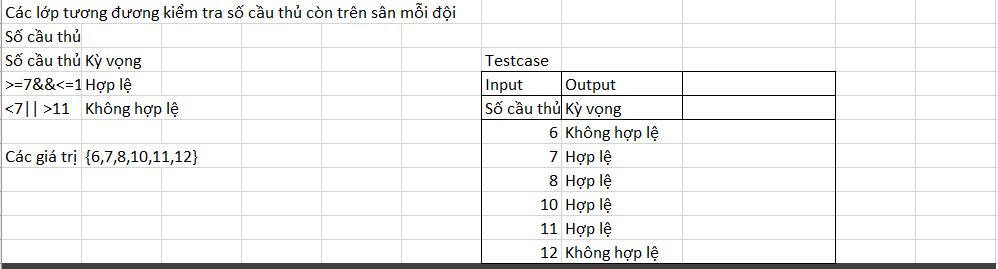
\includegraphics[scale=0.75]{hinh17.png}\\
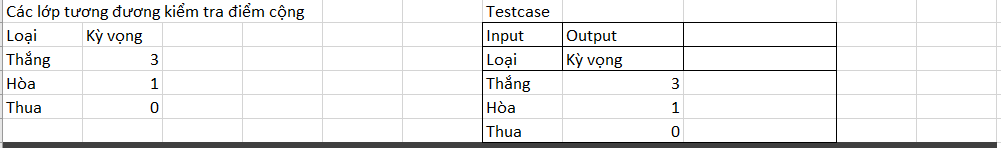
\includegraphics[scale=0.75]{hinh18.png}\\
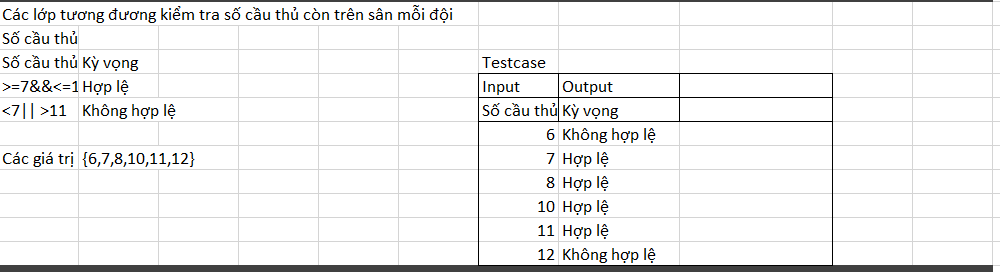
\includegraphics[scale=0.75]{hinh19.png}\\
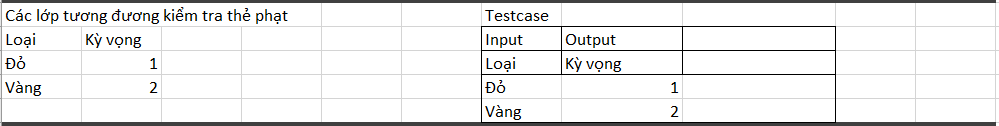
\includegraphics[scale=0.75]{hinhh20.png}\\
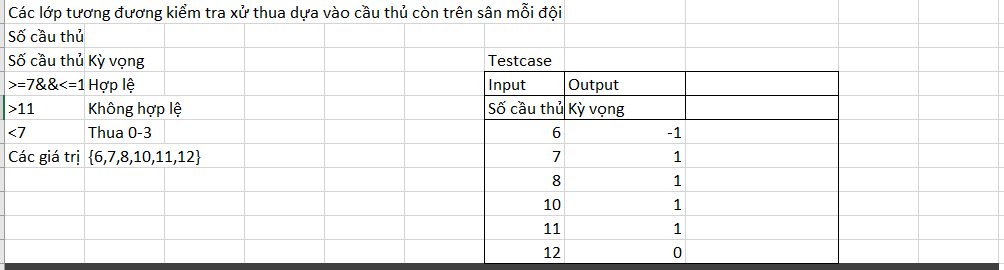
\includegraphics[scale=0.75]{hinh21.png}\\
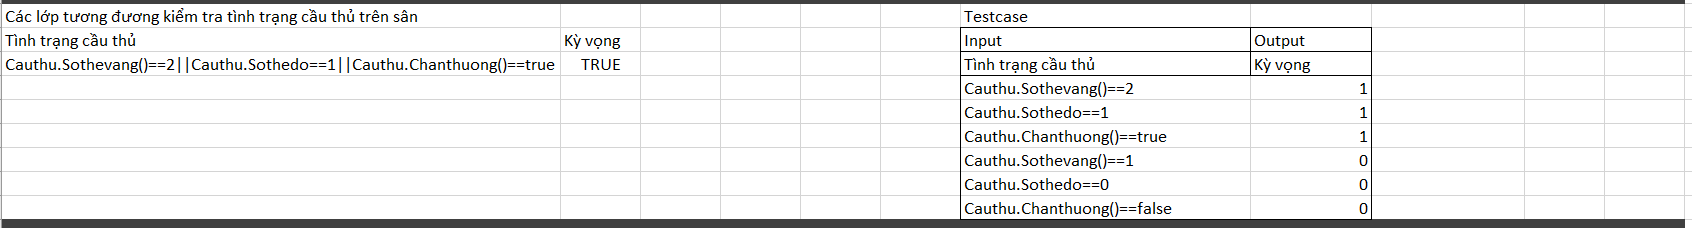
\includegraphics[scale=0.45]{hinh23.png}\\

\section{Kết quả chạy thử chương trình:}\\
\begin{center}
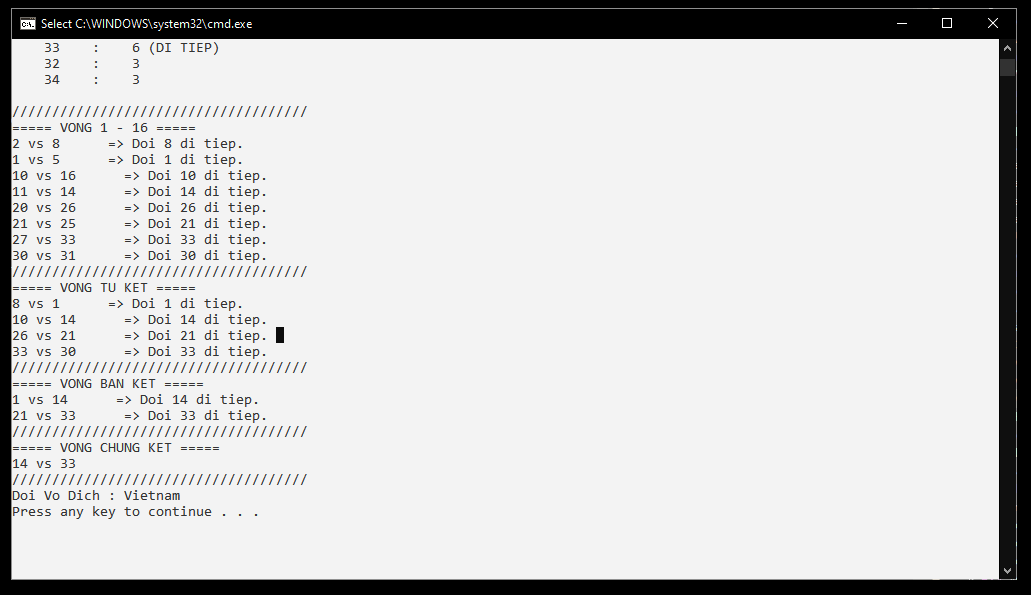
\includegraphics[scale=0.45]{ketqua.png}
\end{center}
\begin{center}
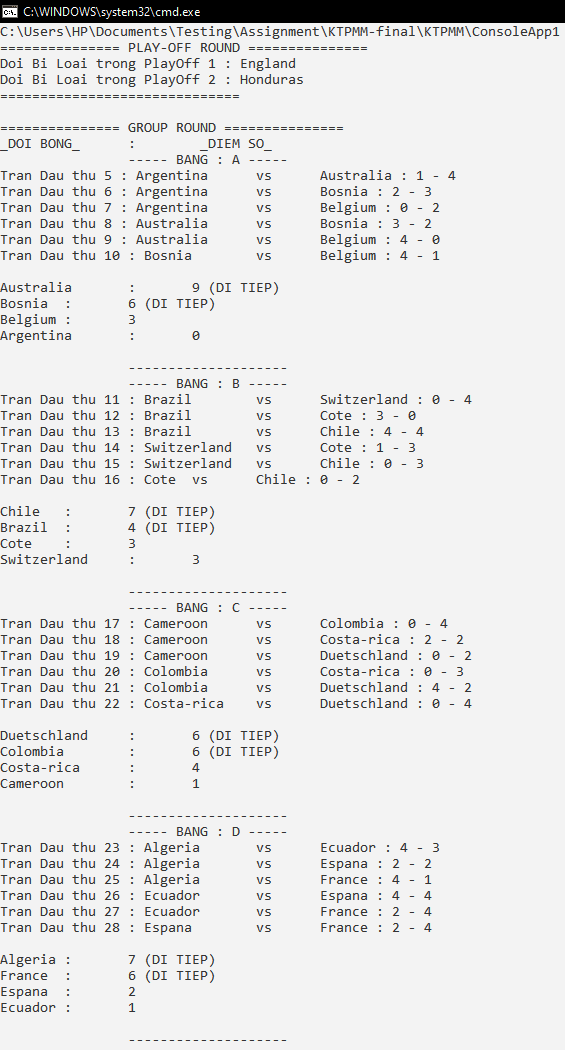
\includegraphics[scale=0.6]{hinh26.png}
\end{center}
\begin{center}
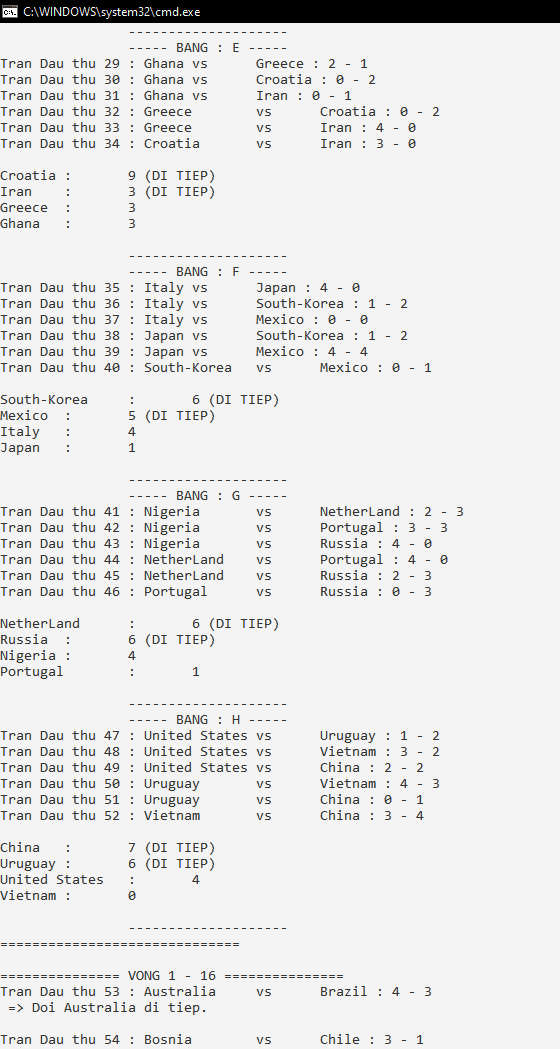
\includegraphics[scale=0.6]{hinh27.png}
\end{center}
\begin{center}
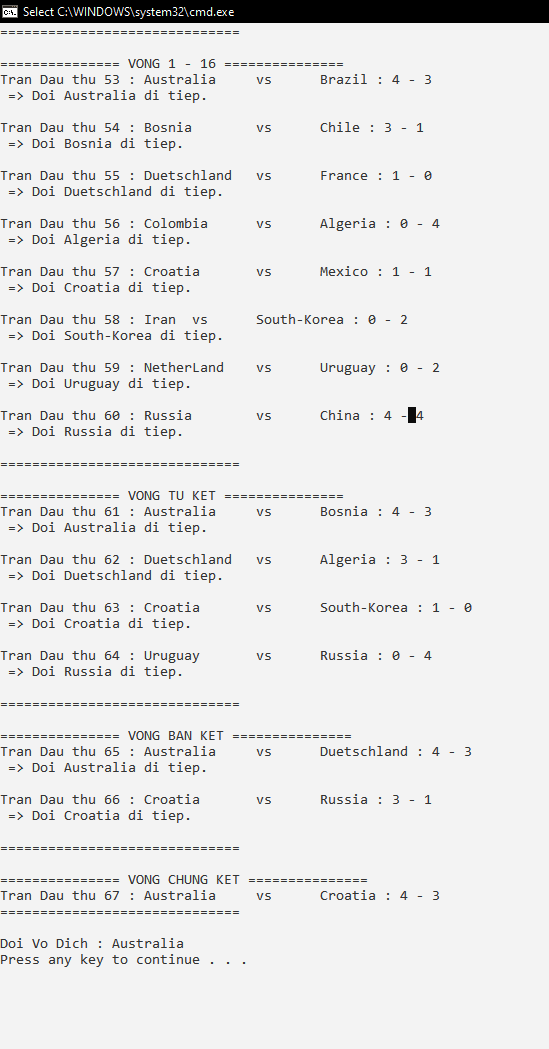
\includegraphics[scale=0.6]{hinh28.png}
\end{center}
\newpage
\textbf{Kết quả kiểm tra độ bao phủ các testcase của nhóm gần như 100\%:}
\begin{center}
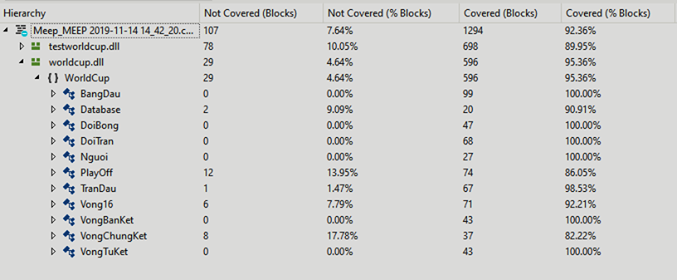
\includegraphics[scale=0.7]{hinh25.png}
\end{center}
\section{Lưu ý khi thực thi chương trình: }\\
Trước khi thực hiện chạy chương trình cần thay đổi đường dẫn của database tại file Database.cs.
\begin{center}
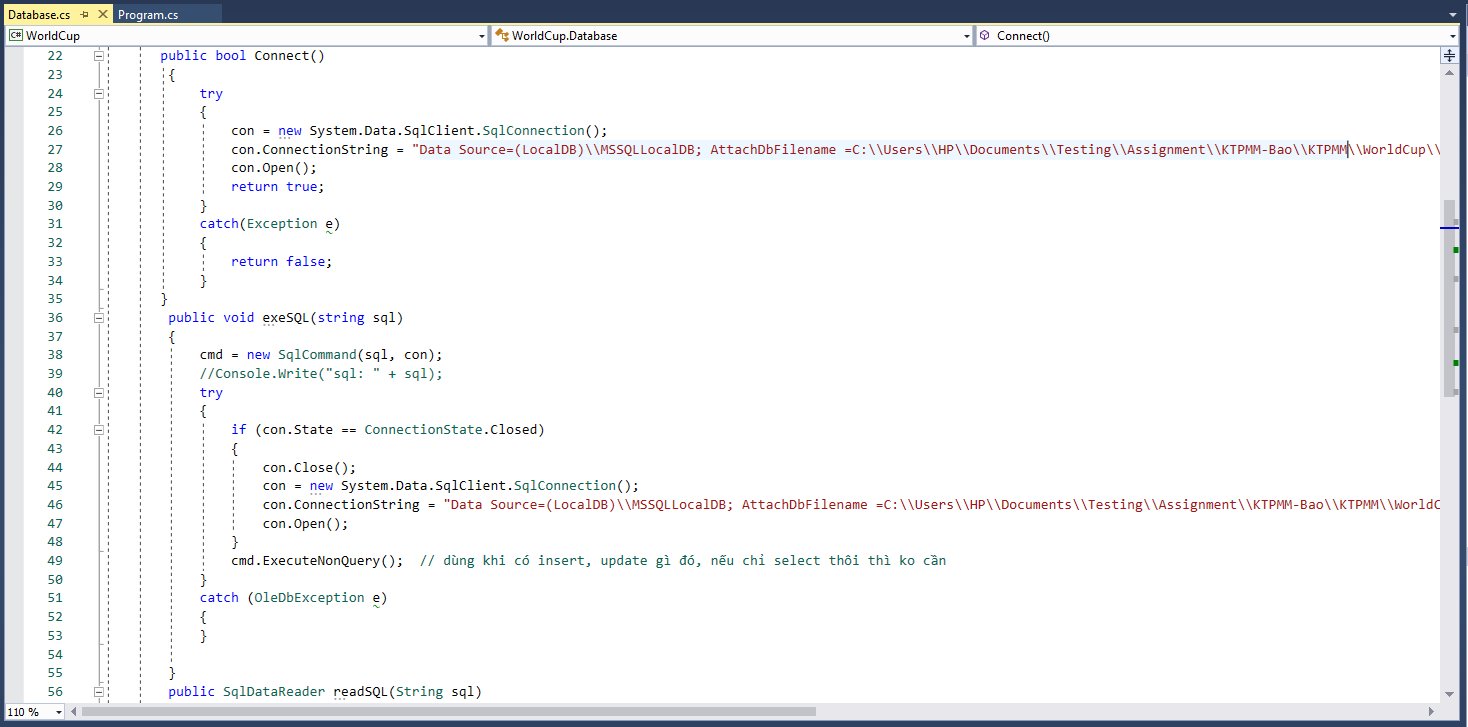
\includegraphics[scale=0.3]{NOTE.png}    
\end{center}
\newpage
\section{Phân chia công việc:}\\
\\

\\
\begin{table}[htbp]
\centering
\begin{tabularx}{\linewidth}{|l|X|}
\hline
\multicolumn{1}{|c|}{\textit{\textbf{STT}}} & \multicolumn{1}{c|}{\textit{\textbf{Công việc}}}                                                   \tabularnewline \hline
Huỳnh Quốc Phú & Phân chia công việc và hiện thực một số class được giao nhiệm vụ.                                                     \tabularnewline \hline
Hy Phạm Ngọc Linh & Viết báo cáo và tạo test case cho hệ thống.                                                      \tabularnewline \hline
Trương Gia Bảo &  Xây dựng DataBase và hiện thực một số class được giao nhiệm vụ.                        \tabularnewline \hline
Trần Minh Tú & tạo test case cho hệ thống và thực hiện một số class được giao nhiệm vụ.\tabularnewline \hline
\end{tabularx}
\end{table}
Tự đánh giá : Hầu hết các công việc đều được cách thành viên trong nhóm thực hiện tốt và tích cực. Các thành viên trong nhóm đều cố gắng đóng góp ý kiến để góp phần hoàn thiện bài tập lớn này. Theo đánh giá cá nhân của nhóm trưởng và tổng hợp các ý kiến của thành viên trong nhóm có thể nói tất cả các thành viên trong nhóm đều hoạt động và làm việc rất tốt trong bài tập lớn này. Tuy nhiên, do khối lượng của bài tập lớn được nhóm đánh giá là khá lớn, đồng thời thời điểm làm bài tập lớn này trùng với một số bài tập lớn khác nên việc sắp xếp thời gian để làm việc nhóm còn khá hạn chế. Từ đó dẫn đến việc nhóm chưa thể hoàn thành 100\% khối lượng công việc được giao trong bài tập lớn.

\begin{thebibliography}{9}
\bibitem{Introduction to Test Driven Development (TDD)}Introduction to Test Driven Development (TDD) : \url{http://agiledata.org/essays/tdd.html}
\bibitem{Unit Test Your Code}Unit Test Your Code :\url{https://docs.microsoft.com/en-us/visualstudio/test/unit-test-your-code?view=vs-2015}
\bibitem{}File báo cáo Latex: \url{https://www.overleaf.com/read/wvsvvxygqdyb}
\end{thebibliography}
\end{document}
